\section{Beweisbarkeit}

\begin{frame}{Der Aussagenkalkül}
	\begin{block}{Was ist ein Kalkül?}
		\begin{itemize}
			\item Ein \emph{Rechensystem}: \; \textbf{Dinge} und was man mit ihnen \textbf{anstellen} darf. \\
			Bsp.: \quad $\R$ und $+, -, \*, /$ \qquad Schachbrett, Figuren und Zugregeln
		\end{itemize}
	\end{block}
	\pause
	\begin{block}{Aussagenkalkül}
		Haben
		\begin{itemize}
			\item Syntaktisch korrekte Formeln $For_{AL}$ \\
			\impl können erfüllbar sein oder nicht 
			\item Davon nennen wir einige bestimmte \textbf{Axiome} \\
			\impl setzen wir als Tautologien voraus
			\item Eine \emph{Schlussregel}: \textbf{Modus Ponens} \\
			...um neue wahre Aussagen zu konstruieren
		\end{itemize}
	\end{block}
\end{frame}

\begin{frame}{Axiome, Modus Ponens}
	\begin{block}{Axiome}
		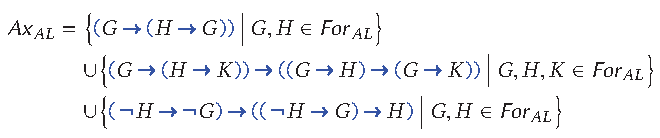
\includegraphics[width=.90\linewidth]{../figures/Axiome} \\
		Wir bestimmen: Das sind unsere „Basis-Tautologien“.
	\end{block}
	\pause
	\begin{block}{Modus Ponens (MP)}
		
		\begin{columns}[T] 
			\begin{column}[T]{.45\textwidth} 
				\vspace{-.6\baselineskip}
				\begin{itemize}
					\item<2-> Wenn $G$ gilt
					\item<2-> und $G \bimp H$ gilt \\ \mbox{}
					\implitem<2-> dann gilt auch $H$.
					\item<4-> Schreibweise: \deduction{G \qquad G \bimp H \concludes H} 
				\end{itemize}
			\end{column}
			\hspace{-2\baselineskip}
			\begin{column}[T]{.55\textwidth} 
				\vspace{-.6\baselineskip}
				\begin{itemize}
					\item<3-> Wir wissen: „Es regnet.“
					\item<3-> Wir erinnern uns: \\ „Wenn es regnet, ist die Straße nass.“
					\implitem<3-> Also wissen wir: „Die Straße ist nass“.
				\end{itemize}
				\hspace{.6\baselineskip} \only<5->{\fbox{\parbox{.9\linewidth}{Mit MP können wir aus bekannten \\ Wahrheiten neue konstruieren!}}}
			\end{column}
		\end{columns}
		
	\end{block}
\end{frame}

\begin{frame}{Ableitungen}
	Haben Formelsammlung $\Gamma$ („Hypothesen“/„Prämissen“), \\
	wollen eine Formel $G$ daraus ableiten
	\pause
	\begin{block}{Ableitung von $G$ aus $\Gamma$}
		Eine „Abfolge“ von Formeln, die in $G$ mündet \quad (Schreibweise: \; $\Gamma \vdash G$) \\
		Was dürfen wir machen?
		\pause
		\begin{itemize}
			\item<+-> aus syntaktisch korrekten Formeln \emph{Axiome} bilden und hinschreiben
			\item<.-> \emph{Prämissen} aus $\Gamma$ hinschreiben
			\item<.-> aus zwei vorherigen Formeln mit \emph{Modus Ponens} eine neue konstruieren
			\implitem<+-> das machen wir solange, bis wir $G$ konstruiert haben
		\end{itemize}
	\end{block}
\end{frame}

\begin{frame}{Ableitungen}
	\begin{exampleblock}{Beispiel}   % geklaut aus 2017 ÜB2 A4
		Gegeben sei die Prämissenmenge $\Gamma = \set{\alA \bimp \alB, \, \alA \bimp \bnot \alB}$ und die Formel $F = \bnot \alA$. \\ 
		Ableitung $\Gamma \vdash F$: \\
		\begin{tabular}{@{}l@{\;\;}l@{\;\;}l}
			1. & $\alA \bimp \alB$ & Prämisse 1; ist $\in \Gamma$ \\
			2. & $\alA \bimp \bnot \alB$ & Prämisse 2; ist $\in \Gamma$ \\
			3. & $\alka \alA \bimp \alB \alkz \bimp \alka \alka \alA \bimp \bnot \alB \alkz \bimp \bnot \alA \alkz$ & Anwendung von $Ax_{AL3}$ {\small (mit $H = \bnot \alA$ und $G = \bnot \alB$)} \\ 
			& & ({\small  Schema $Ax_{AL3}$:  $\alka \bnot H \bimp \bnot G \alkz \bimp \alka \alka \bnot H \bimp G \alkz \bimp H \alkz $ }) \\
			4. & $\alka \alA \bimp \bnot \alB \alkz \bimp \bnot \alA $ & MP (3, 1) \quad {\small (Modus Ponens mit Formeln 3 und 1)} \\
			5. & $\bnot \alA$ & MP (4, 2) \quad {\small (Modus Ponens mit Formeln 4 und 2)} \\
		\end{tabular}
	\end{exampleblock}
\end{frame}

\begin{frame}{Beweisbarkeit}
	\begin{block}{Beweis von $G$}
		\impl Ableitung von $G$ aus $\Gamma  = \emptyset$ \\
		\impl Wir verwenden nur Axiome und MP, es gibt \textbf{keine} Prämissen! \\
		Schreibweise: \quad $\vdash G$ \qquad „$G$ ist beweisbar“ \\
		Ein solches beweisbares $G$ nennen wir \textbf{Theorem} des Kalküls.
	\end{block}
	\pause 
	\begin{block}{Lemma}
		Eine AL-Formel $G$ ist genau dann Tautologie, wenn $G$ ein Theorem des AL-Kalküls ($=$~im Kalkül beweisbar) ist. \\
		\smallskip
		\centered{--- bzw. ---} 
		\smallskip
		Für jede AL-Formel $G$ gilt: \qquad $\models G \; \Gdw \; \vdash G$.\\
	\end{block}
	(Achtung: Es gibt Kalküle / Logiken, für die so etwas nicht gilt!)
	\pause
	\begin{block}{Lemma}
		Für Formeln $G$, $H$ gilt $G \vdash H$ genau dann, wenn $\vdash \bleftBr G \bimp H \brightBr$.
	\end{block}
\end{frame}
